\chapter{Proof for rank 4}
\label{proof-4}

\paragraph{}
We study the different cases for polytopes of rank 4. By Lemma~\ref{min-4-trans}, we can have two, three or four 4-transposition.

\section{Preliminary results}

\begin{theorem}
  Neither $\rho_1$ nor $\rho_2$ can be 2-transposition.
\end{theorem}

\begin{proof}
  Suppose that $\rho_2$ is a 2-transposition. They must be at least two 4-transpoistions out of the three other involutions. Therefore $\rho_2$.
  $\rho_2$ ou $\rho_3$ est une 4-transposition. Donc $\rho_0$ doit partager des sommets avec au moins une d'entre elle.

  \paragraph{}
  Si c'est $\rho_2$ qui est une 4-transposition, $\rho_0$ et $\rho_3$ doivent partager un sommet. Dès lors, elles doivent former soit un carré alterné $[\rho_0, \rho_3]$ soit une arête double $(\rho_0, \rho_3)$.

  \paragraph{}
  Dans le premier cas, ce carré alterné devra être adjacent à un autre carré alterné $[\rho_0, \rho_2]$, dans le second cas, on a le choix entre ce carré et un carré du type $[\rho_1, \rho_3]$. Dans les deux cas, nous avons utilisés toutes nos arêtes exédentaires, la suite devra donc être linéaire. En fonction des cas que nous avons faits, il y a trois possibiliés:

  \begin{itemize}
    \item 1 $\rho_0$, 2 $\rho_1$, 2 $\rho_2$, 0 $\rho_3$
    \item 2 $\rho_0$, 2 $\rho_1$, 2 $\rho_2$, 1 $\rho_3$
    \item 3 $\rho_0$, 0 $\rho_1$, 4 $\rho_2$, 0 $\rho_3$
  \end{itemize}

  \paragraph{}
  Le troisième cas est clairement impossible car, en partant d'une arête $\rho_2$, nous ne pourons jamais atteindre $\rho_0$ de manière linéaire.

  \paragraph{}
  Dans les deux premiers cas, nous devons continuer avec des arêtes $\rho_1$ donc le trois

\end{proof}

\paragraph{}
We start by proving some lemmas that are used when there are used for the cases with three or four 4-transpositions. We suppose in the following proofs that if there is a 2-transition, then it is $\rho_0$. This can be done with the previous theorem and by using the duality.

\begin{lemma}
  In a sggi $\Gamma$ of rank 4 on $A_{11}$ with at least three 4-transpositions, there must be a least one single $\rho_1$ edge (and thus a single $\rho_3$ edge).
\end{lemma}

\begin{proof}
  By Lemma~\ref{adjacent-must-not-commute}, a $\rho_0$ must be adjacent to a $\rho_1$ edge. The $\rho_1$ can be a single edge, a double edge with another involution or on an alternating square.

  \paragraph{}
  If the $\rho_1$ edge is part of a double edge then the other involution of this double edge can be $\rho_2$ or $\rho_3$. But if the $\rho_0$ and $\rho_1$ do not commute then $\rho_0$ does not commute with the other involution and this is a contradiction with Proposition~\ref{intersection-patterns}.

  \paragraph{}
  If $\rho_1$ is on an alternating square, the same occurs\footnote{More precise}.

\end{proof}

\begin{lemma}
  There cannot be more than one $\rho_1$ single edge and thus there cannot be more than one $\rho_3$ single edge.
\end{lemma}

\begin{proof}
  There are not enough points otherwise. Hence if they are two single $\rho_1$ edges, there are two single $\rho_3$ edges. Those 4 edges uses 8 points. The four last edges can be arranged in an alternating square or two double edges. Those edges uses 4 vertices. That is not possible because there are only 11 points.
\end{proof}

\begin{corollary}
  \label{rank-4-single-1}
  There are exactly one $\rho_1$ single edge and one $\rho_3$ single edge.
\end{corollary}

\begin{lemma}
  \label{rank-4-3-patterns}
  Let $\Gamma$ be a sggi of rank 4 on 11 points. If $\rho_1$, $\rho_2$ and $\rho_3$ are 4-transpositions then the patterns formed by $\rho_1$ and $\rho_3$ edges are one alternating square, one double edge and two simple edges (one for each involution).
\end{lemma}

\begin{proof}
  By Corollary~\ref{rank-4-single-1} there is exactly one $\rho_1$ single edge. The remaining possibilities for the three remaining edges of $\rho_1$ are limited: one alternating square $[\rho_1, \rho_3]$ and one double edge $(\rho_1, \rho_3)$ or three double edges $(\rho_1, \rho_3)$.

  \paragraph{}
  Suppose that there are three double edges.

    \begin{figure}[H]
      \begin{center}
        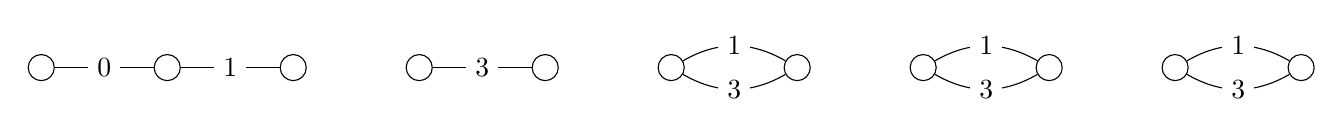
\begin{tikzpicture}[scale=.8]

          \begin{scope}[every node/.style={circle,draw}]
            \node (1)  at (0,0)  {};
            \node (2)  at (2,0)  {};
            \node (3)  at (4,0)  {};
            \node (4)  at (6,0) {};
            \node (5)  at (8,0)  {};
            \node (6)  at (10,0)  {};
            \node (7)  at (12,0)  {};
            \node (8)  at (14,0)  {};
            \node (9)  at (16,0)  {};
            \node (10) at (18,0)  {};
            \node (11) at (20,0)  {};
          \end{scope}

          \begin{scope}[every node/.style={fill=white}]

            \begin{scope}[every edge/.style={draw}]
              \path (1)  edge node {$0$} (2);
              \path (2)  edge node {$1$} (3);
              \path (6)  edge[bend left=30] node {$1$} (7);
              \path (8)  edge[bend left=30] node {$1$} (9);
              \path (10) edge[bend left=30] node {$1$} (11);
              \path (4)  edge node {$3$} (5);
              \path (6)  edge[bend right=30] node {$3$} (7);
              \path (8)  edge[bend right=30] node {$3$} (9);
              \path (10) edge[bend right=30] node {$3$} (11);
            \end{scope}
          \end{scope}

        \end{tikzpicture}
        \caption{}
      \end{center}
    \end{figure}

  \paragraph{}
  By~\ref{todo}\footnote{Not complete}, no other $\rho_0$ edge can be placed.
\end{proof}
